%-*- coding: UTF-8 -*-
% notes.tex
%
\documentclass[UTF8]{article}
\usepackage{geometry}
\geometry{a4paper, centering, scale=0.8}
\usepackage{minted}
\usepackage{hyperref}
\usepackage{indentfirst}    % to indent the first paragraph of a section
\usepackage{graphicx}       % to insert figures
\usepackage{amsmath}        % to type some math equations
\usepackage{amssymb}        % to use some special math font
\usepackage{IEEEtrantools}  % to use IEEEeqnarray
\usepackage{algorithm2e}    % to use algorithm environment
\usepackage{multicol}       % to display some content in multi-columns
\setlength{\columnseprule}{0.4pt}   % set the rule's width of multicols
\setlength{\columnsep}{5em}         % set the sep of multicols

% Math notation
% refered to https://github.com/exacity/deeplearningbook-chinese/blob/master/math_symbol.tex
\newcommand{\Scalar}[1]{\mathit{#1}}                % Scalar, the default math font
\newcommand{\Vector}[1]{\boldsymbol{\mathit{#1}}}   % Vector
\newcommand{\Matrix}[1]{\boldsymbol{\mathit{#1}}}   % Matrix
\newcommand{\Tensor}[1]{\textsf{\textbf{#1}}}       % Tensor
\newcommand{\Set}[1]{\mathbb{#1}}                   % Set
\newcommand{\Cal}[1]{\mathcal{#1}}                  % Math Cal

% Draw the lines in a matrix, which is composed by a series of vectors
\newcommand{\vRule}{\rule{0.3pt}{10mm}}             % vertical rule
\newcommand{\hRule}{\,\rule[1mm]{10mm}{0.3pt}\,}    % horizontal rule

\title{Deep Learning Specialization \\
        Improving Deep Neural Networks: Hyperparameter tuning, Regularization and Optimization \\
        Learning Notes}
\author{Du Ang \\ \texttt{du2ang233@gmail.com} }
\date{\today}

\begin{document}
\maketitle

\tableofcontents
\newpage

\section{Practical aspects of Deep Learning}
\subsection{Setting up your Machine Learning Application}
\subsubsection{Train/Dev/Test sets}
When training a neural network, you have to make a lot of decisions, such as choosing the number of
layers of the neural network, choosing the number of hidden units of each hidden layer, choosing
the learning rates and activations.

Applied machine learning is a highly iterative process. At first, you have some ideas and make some
decisions. Then you implement the ideas with code in programming. You run some experiments and you
get back a result that tells you how well this particular network, or this particular configuration
works. And based on the outcome, you might refine your ideas and change your choices and maybe keep
iterating in order to try to find a better and beter neural network.

Intuitions from one domain or from one application area often do not transfer to other application
areas. And the best choices may depend on the amount of data you have, the number of input features
you have through your computer configuration and whether you're training on GPUs or CPUs. Even very
experienced deep learning people find it almost impossible to correctly guess the best choice of
hyperparameters the very first time. And so today, applied deep learning is a very iterative
process where you just have to go around this cycle many times to hopefully find a good choice of
network for your application. So one of the things that determine how quickly you can make progress
is how efficiently you can go around this cycle.

Setting up your data sets well in terms of your train, development and test sets can make you much
more efficient at that. The dataset can be separated into three parts: training set, dev set
(development set, hold-out cross validation) and test set.

In the previous era of machine learning, it was common practice to take all your data and split it
accordin to 70/30 percent in terms of a people often talk about the 70/30 train test splits, if you
don't have an explicit dev set. Or maybe a 60/20/20 percent split in terms of 60\% train, 20\% dev
and 20\% test. And several years ago, this was the widely considered as the best practice in
machine learning, if you have 100, 1000 or 10,000 examples.

But in modern big data era, where you might have a million examples in total, then the trend is
that your dev and test sets have been becoming a much smaller percentage of the total. Because
remember, the goal of the dev set is that you're going to test different algorithms on it and see
which algorithm choices works better. So the dev set just needs to to be big enough for you to
evaluate, for example, two different algorithm choices or ten different algorithm choices and
quickly decide which one is doing better. And you might not need a whole 20\% of your data for that.
Similarly, the main goal of your test set is, given your final classifier, to give you a pretty
confident estimate of how well it's doing.

\begin{description}
    \item[Previous era (small exampels): ] training set/dev set/test set : 60/20/20
    \item[Big data era: ] training set/dev set/test set : 98/1/1
\end{description}

One other trend we're seeing in the era of modern deep learning is that more and more people train
on mismatched train and test distributions. Let's say you're building an app that lets users upload
a lot of pictures and your goal is to find pictures of cats in order to show your users. Maybe all
your training set comes from cat pictures downloaded off the Internet, but your dev and test sets
might comprise cat pictures from user using our app. It turns out that a lot of webpages have very
high resolution, very professional, very nicely framed pictures of cats. But maybe your users are
uploading blurrier, lower resolution images just taken with a cell phone camera in a more casual
condition. And so the two distributions of data may be different. The rule of thumb to follow in
this case is to make sure that the dev and test sets come from the same distribution.

Finally, it might be okay to not have a test set. If you have only a dev set but not a test set,
what you do is you train on the training set and then try different model architectures. Evaluate
them on the dev set, and then use that to iterate and try to get to a good model. Because you've
fit your data to the dev set, this no longer gives you an unbiased estimate of performance.

In machine learning world, when you have just a train and a dev set but no separate test set, most
people will call this a training set and they will call the dev set the test set. But what they
actually end up doing is using the test as a hold-out cross validation set. Which maybe isn't
complete a great use of terminology, because they're overfitting to the test set.

Having set up a train dev and test set will allow you to integrate more quickly. It will also allow
you to more efficently measure the bias and variance of your algorithm, so you can more efficiently
select ways to improve your algorithm.

\subsubsection{Bias/Variance}
\begin{figure}[htb]
    \centering
    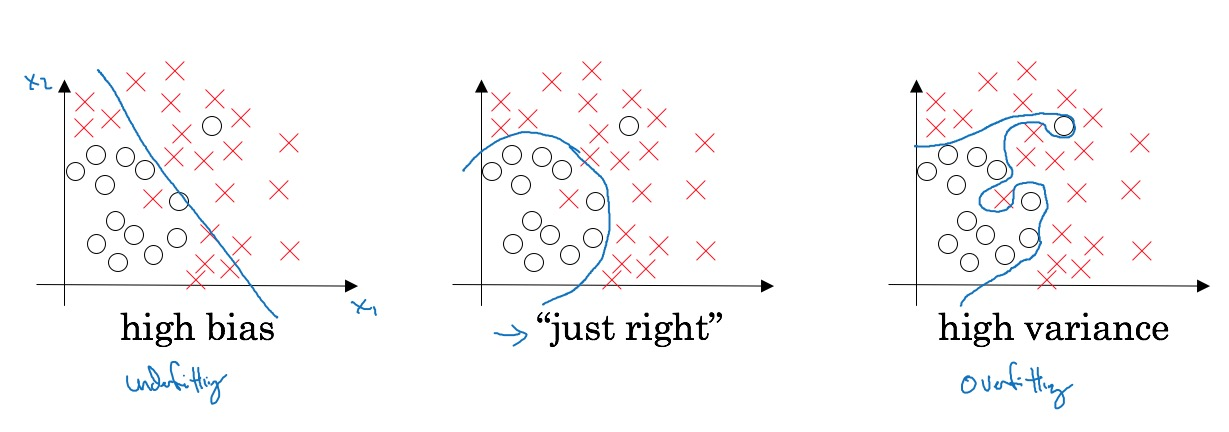
\includegraphics[width=40em]{figures/bias-and-variance-1}
    \caption{Decision boundaries of different classifier on 2D examples}
\end{figure}

\begin{figure}[htb]
    \centering
    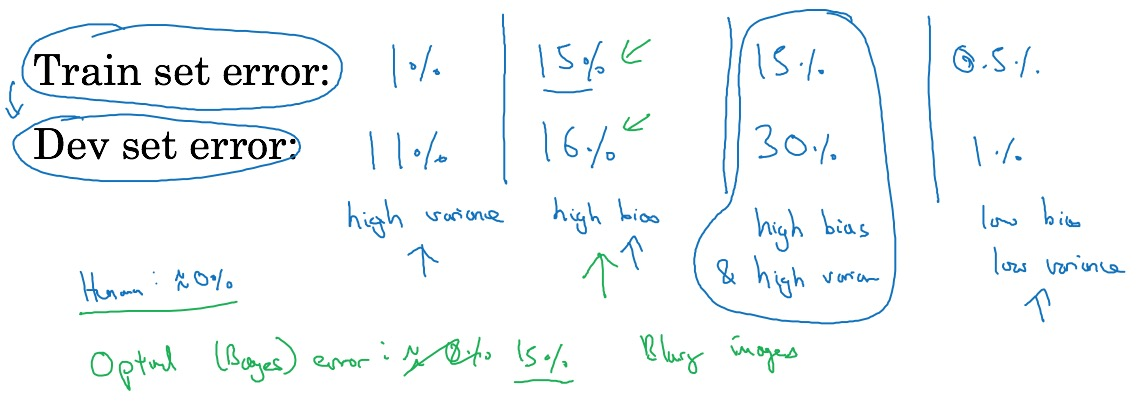
\includegraphics[width=40em]{figures/bias-and-variance-2}
    \caption{Bias or Variance showed by training set error and dev set error. It is related to the
    optimal error (Bayes error), which is determined by the common practices and our expectation.}
\end{figure}

\begin{figure}[htb]
    \centering
    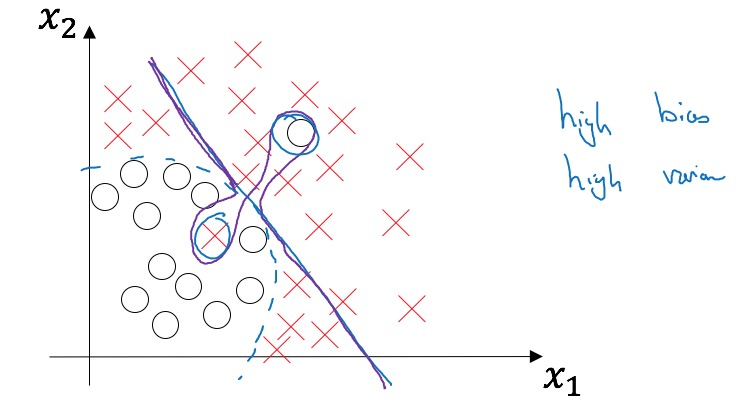
\includegraphics[width=30em]{figures/bias-and-variance-3}
    \caption{The purple decision boundary shows a high bias and high variance case}
\end{figure}

\subsubsection{Basic Recipe for Machine Learning}
\begin{figure}[htb]
    \centering
    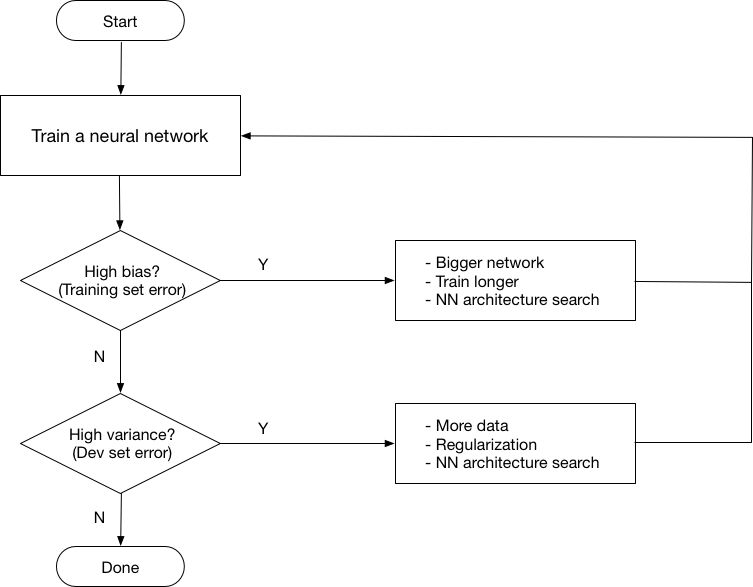
\includegraphics[width=30em]{figures/machine-learning-recipe}
    \caption{Basic recipe for Machine Learning}
    \label{fig:machine-learning-recipe}
\end{figure}

Whereas getting a bigger network almost always helps, and training longer doesn't always help, but
it certainly never hurts. Usually if you have a big enough network, you should usually fit the
training data well so long as it's problem that is possible for someone to do.

If you have high variance problem, the best way to solve high variance problem is to get more data.
But sometimes you can't get more data, or you could try regularization to reduce overfitting. But
if you can find a more appropriate neural network architecture, sometimes that can reduce your
variance problem as well, as well as reduce your bias problem.

Like Figure~\ref{fig:machine-learning-recipe} shows, there are a couple of points to notice. First
is that, depending on whether you have high bias or high variance, the set of things hou should try
could be quite different. So usually use the training dev set to try to diagnose if you have a bias
or variance problem, and then use that to select the appropriate subset of things to try. So for
example, if you actually have a high bias problem, getting more training data is actually not going
to help. Or at least it's not the most efficient thing to do.

\paragraph{Bias variance trade-off} In the earlier era of machine learning, there used to be a lot
of discussion on what is called the bias variance trade-off. And the reason for that was that, for
a lot of the things you could try, you could increase bias and reduce variance, or reduce bias and
increase variance. Back in the pre-deep learning era, we didn't have many tools, we didn't have
as many that just reduce bias or that just reduce variance without hurting the other one. But in
the modern deep learning, big data era, so long as you can keep training a bigger network, and so
long as you can keep getting more data, which isn't always just reduces your bias without
necessarily hurting your variance, so long as you regularize appropriately. And getting more data
always reduces your variance and doesn't hurt your bias much. So what's really happened is that,
with these two steps, the ability to train, pick a network, or get more data, we now have tools to
drive down variance, without really hurting the other thing that much.

\subsection{Regularizing your neural network}
\subsubsection{Regularization}
If you suspect your neural network is overfitting your data, that is you have a high variance
problem, one of the first thing you should try is probably regularization. The other way to address
high variance is to get more training data, which is also quite reliable, but you can't always get
more training data, or it could be more expensive to get more data. But adding regularization
will often help to prevent overfitting, or to reduce the errors in your network.

\paragraph{Logistic regression}
$$ \underset{\Vector{w}, b}{\text{min}} J(\Vector{w}, b) \qquad
\Vector{w} \in \Set{R}^{n_x}, b \in \Set{R} $$
$$ J(\Vector{w}, b) = \frac{1}{m} \sum_{i=1}^m \Cal{L}(\hat{y}^{(i)}, y^{(i)})
+ \frac{\lambda}{2m} ||\Vector{w}||_2^2 $$

\begin{description}
    \item[$L_2$ Norm (squared)]
    $\displaystyle ||\Vector{w}||_2^2 = \sum_{j=1}^{n_x} \Vector{w}_j^2 = \Vector{w}^T \Vector{w} $
    \item[$L_1$ Norm]
    $\displaystyle ||\Vector{w}||_1 = \sum_{j=1}^{n_x}|\Vector{w}_j| $ \qquad
    (Using $L_1$ Norm will make $\Vector{w}$ sparse)
\end{description}

The $\lambda$ means ``regularization parameter'', it helps prevent overfitting. In Python,
\mintinline{python}{lambda} is a reserved keyword, so we use \texttt{lambd}, without \texttt{a}, to
represent the lambda regulzarization parameter.

\paragraph{Neural network}
$$ J(\Matrix{W^{[1]}}, \Vector{b^{[1]}}, \ldots, \Matrix{W}^{[L]}, \Vector{b}^{[L]})
= \frac{1}{m} \sum_{i=1}^{m} \Cal{L}(\hat{\Vector{y}}^{(i)}, \Vector{y}^{(i)})
+ \frac{\lambda}{2m} \sum_{l=1}^L ||\Matrix{W}^{[l]}||_F^2 \qquad
\Matrix{W} \in \Set{R}^{(n^{[l]}, n^{[l-1]})}$$

\begin{description}
    \item[Frobenius Norm (squared)]
    $ \displaystyle ||\Matrix{W}^{[l]}||_F^2 = \sum_{i=1}^{n^{[l-1]}} \sum_{j=1}^{n^{[l]}}
    (\Matrix{W}_{ij})^2 $ \\ (the sum of squares of elements of a matrix, just like $L_2$ norm)
\end{description}

In backpropagation,
$$ \text{d}\Matrix{W}^{[l]} = \frac{1}{m} \text{d}\Matrix{Z}^{[l]} {\Matrix{A}^{[l-1]}}^T
+ \frac{\lambda}{m} \Matrix{W}^{[l]} $$
$$ \Matrix{W}^{[l]} := \Matrix{W}^{[l]} - \alpha \text{d}\Matrix{W}^{[l]} $$

$L_2$ norm sometimes is called ``weight decay'', that's because
\begin{IEEEeqnarray*}{rCl}
\Matrix{W}^{[l]} := \Matrix{W}^{[l]} - \alpha \text{d}\Matrix{W}^{[l]}
= \Matrix{W}^{[l]} - \alpha (\frac{1}{m} \text{d}\Matrix{Z}^{[l]} {\Matrix{A}^{[l-1]}}^T
+ \frac{\lambda}{m} \Matrix{W}^{[l]})
= (1 - \frac{\alpha \lambda}{m}) \Matrix{W}^{[l]}
- \frac{\alpha}{m} \text{d}\Matrix{Z}^{[l]}{\Matrix{A}^{[l-1]}}^T
\end{IEEEeqnarray*}

\subsubsection{Why regularization reduces overfitting?}
\paragraph{Intuition 1}
$$ J(\Matrix{W^{[1]}}, \Vector{b^{[1]}}, \ldots, \Matrix{W}^{[L]}, \Vector{b}^{[L]})
= \frac{1}{m} \sum_{i=1}^{m} \Cal{L}(\hat{\Vector{y}}^{(i)}, \Vector{y}^{(i)})
+ \frac{\lambda}{2m} \sum_{l=1}^L ||\Matrix{W}^{[l]}||_F^2 $$

What we did for regularization was adding extra term $\lambda$ to penalize the weight matricies
$\Matrix{W}^{[l]}$ from being too large. So why is it that shrinking the $L_2$ norm or the
Frobenius norm might cause less overfitting? One piece of intuition is that if you crank
regularization lambda to be really, really big, they'll be really incentivized to set the weight
matricies $\Matrix{W}^{[l]}$ to be reasonably close to zero. So one piece of intuition is maybe it
set the weight to be so close to zero for a lot of hidden units that's basically zeroing out a lot
of the impact of these hidden units. And if that's the case, then this much simplified neural
network becomes a much smaller neural network. In fact, it is almost like logistic regression
units, but stacked most probably as deep. And so that will take you from this overfitting case much
closer to the left to other high bias case, just like Figure~\ref{fig:regularization-intuition-1}.
But hopefully there'll be an intermediate value of lambda that results in a result closer to this
just right case in the middle.

\begin{figure}[htb]
    \centering
    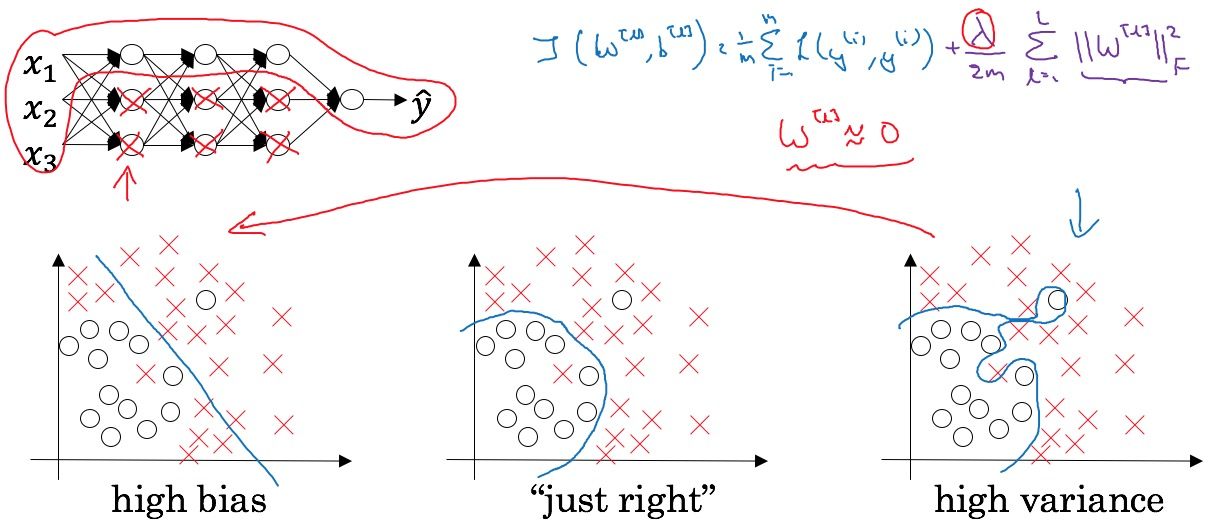
\includegraphics[width=40em]{figures/regularization-intuition-1}
    \caption{A intuition of regularization: big $\lambda$ penalizes weights to almost zeros, make
    it a simpler network}
    \label{fig:regularization-intuition-1}
\end{figure}

\paragraph{Intuition 2}
\begin{figure}[htb]
    \centering
    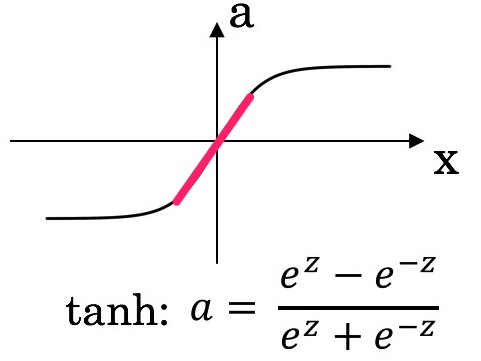
\includegraphics[width=25em]{figures/regularization-intuition-2}
    \caption{A intuition of regularization: big $\lambda$ penalizes weights $\Matrix{W}^{[l]}$
    smaller, then $\Matrix{Z}^{[l]}$ will be smaller and will fall on the linear part of tanh
    activation function}
    \label{fig:regularization-intuition-2}
\end{figure}

In Figure~\ref{fig:regularization-intuition-2}, there is another attempt at additional intuition
for why regularization helps prevent overfitting. And for this, We assume taht we're using the tanh
activation function which looks like this. So if that's the case, if the regularization parameter
$\lambda$ is large, then your parameters $\Matrix{W}^{[l]}$ will be relatively small, then
$\Matrix{Z}^{[l]}$ will be relatively small. And in particular, if $\Matrix{Z}^{[l]}$ ends up
taking relative small values, then $g(\Matrix{Z}^{[l]})$ will be roughly linear. So it's as if
every layer will be roughly linear. We saw in course one that if every layer is linear then your
whole network is just a linear network, as if it is just linear regression. So even a very deep
network, in this case, it will compute something not far from a big linear function which is
therefore pretty simple function rather than a very complex highly non-linear function. And so it
is much less able to overfit.

\subsubsection{Dropout Regularization}
In addition to $L_2$ regularization, another very powerful regularization techniques is called
``dropout''.

Like Figrure~\ref{fig:dropout} shows, with dropout, what we're going to do is go through each of
the layers of the network and set some probability of eliminating a node in neural network. So you
end up with a much smaller, really much diminished network. On different examples, you would toss a
set of coins again and keep a different set of nodes and then dropout or eliminate different set of
nodes. So for each example, you would train it using one of these neural reduced networks.

\begin{figure}[htb]
    \centering
    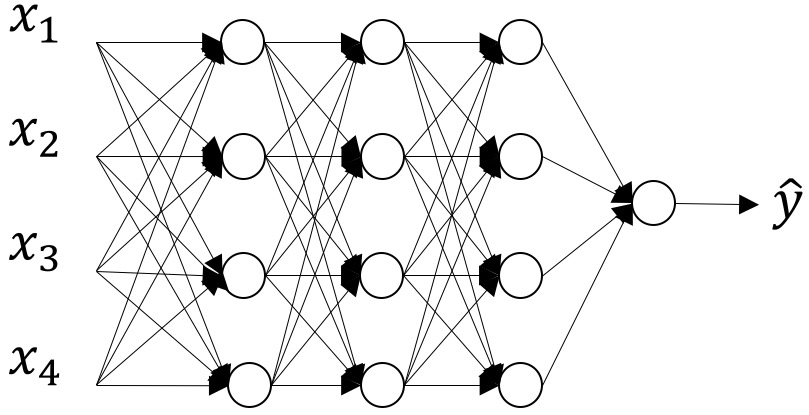
\includegraphics[width=20em]{figures/dropout-orig}
    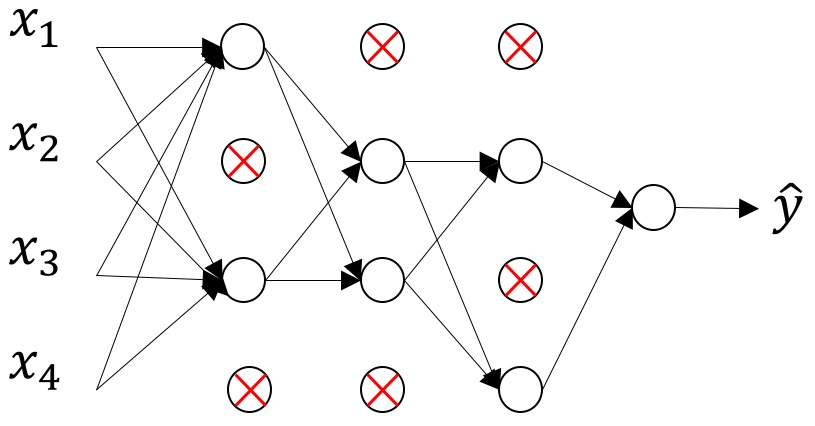
\includegraphics[width=20em]{figures/dropout-zero-out}
    \caption{Dropout}
    \label{fig:dropout}
\end{figure}

\paragraph{Implementing dropout (``Inverted dropout'')}
For the sake of completeness, let's say we want to illustrate this with layer $l=3$. What we are
going to do is set a vector \texttt{d3}, which is going to be the dropout vector for the
layer 3.
\begin{minted}{numpy}
    keep_prob = 0.8  # the probability of keeping each unit

    d3 = np.random.rand(a3.shape[0], a3.shape[1]) < keep_prob
    a3 = np.multiply(a3, d3)  # a3 * d3, element-wise multiplication
    a3 /= keep_prob  # inverted dropout
\end{minted}

\paragraph{Making predictions at test time}
Don't use dropout at test time. That's because when you are making predictions at the test time,
you don't really want your output to be random. If you are implementing dropout at test time, that
just add noise to your predictions. In theory, one thing you could do is run a prediction process
many times with different hidden units randomly dropped out and have it across them. But that's
computationally inefficient and will give you roughly the same result.

And just to mention, the inverted dropout thing, you remember the step on the previous line when we
divided by the \texttt{keep\_prob}. The effect of that was to ensure that even when you don't
implement dropout at test time to the scaling, the expected value of the activations don't change.
So you don't need to add an extra funny scaling parameter at test time.

\subsubsection{Understanding dropout}
Intuition: Can't rely on any one feature, so have to spread out weights. And by spreading norm of
the weights, this will tend to have an effect of shrinking the squared norm of the weights. And so,
similar to what we saw with $L_2$ regularization, the effect of implementing dropout is that it
shrinks the weights and does similar to $L_2$ regularization that helps prevent overfitting.
But it turns out that dropout can formally be shown to be an adaptive form without a regularization,
while $L_2$ penalty on different weights are different, depending on the size of the activations
being multiplied that way.

It is also feasible to vary \texttt{keep\_prob} by layer. The \texttt{keep\_prob} of $1.0$ means
that you're keeping every unit and so you're really not using dropout for that layer. But for
layers where you're more worried about overfitting, really the layers with a lot of parameters, you
can set the \texttt{keep\_prob} to be smaller to apply a more powerful form of dropout.

And technicall, you can also apply droput to the input layer, where you can have some chance of
just maxing out one or more of the input features. Although in practice, usually don't do that that
often. And so, a \texttt{keep\_prob} of $1.0$ was quite common for the input layer.

One downside of dropout is, this gives you even more hyperparameters to search for using
cross-validation. One other alternative might be to have some layers where you apply dropout and
some layers where don't apply dropout, and then you just have one hyperparameter, which is a
\texttt{keep\_prob} for the layers for which you do apply dropouts.

Many of the first successful implementations of dropout were to computer vision, and it is
frequently used by computer vision. But the really thing to remember is that dropout is a
regularization technique, it helps prevent overfitting, don't use it unless your algorithm is
overfitting.

Another big downside of dropout is that the cost function $J$ is no longer well-defined. On every
iteration, you are randomly killing off a bunch of nodes. And so, if you are double checking the
performance of gradient descent, it will be harder to double check that because the cost function
$J$ is less well-defined or is certainly hard to calculate. So we lose the debugging tool to plot
the graph $J$ of the number of iterations. We can turn off dropout (set \texttt{keep\_prob} equals
$1.0$) at first, and run the code to make sure that it is monotonically decresing $J$. Then turn on
dropout and use other ways, but not plotting the figures, to make sure that our code is working,
the gradient descent is working even with dropout.

\subsubsection{Other regularization methods}
\paragraph{Data augmentation}
Let's say you are fitting a cat classifier. If you are overfitting, getting more data can help, but
getting more training data can be expensive and sometimes you just can't get more data. Then like
Figure~\ref{fig:data-augmentation} shows, we can use data augmentation by using flipping, random
cropping, distortion, etc. to get more training data.

\begin{figure}[htb]
    \centering
    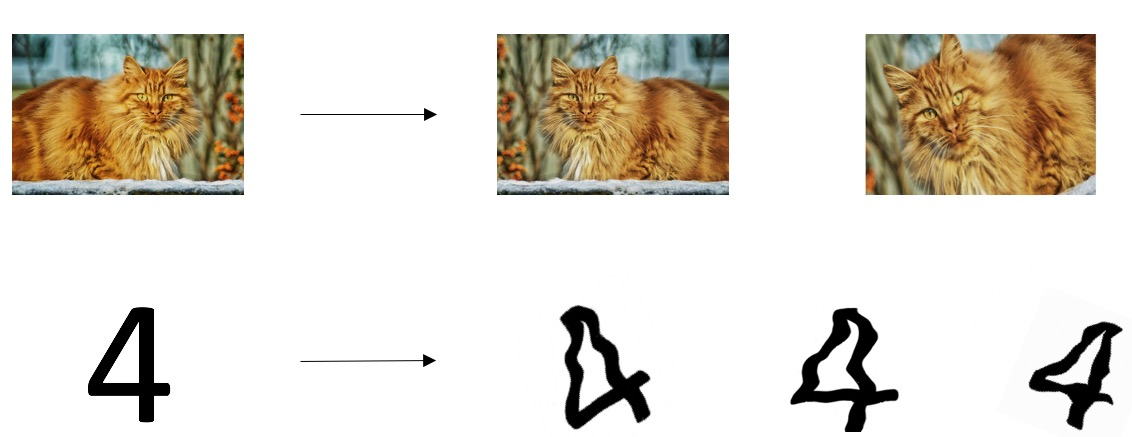
\includegraphics[width=40em]{figures/data-augmentation}
    \caption{Data augmentation}
    \label{fig:data-augmentation}
\end{figure}

\paragraph{Early stopping}
Just like Figure~\ref{fig:early-stopping} shows, what you are going to do is as you run gradient
descent you are going to plot the training error or $J$, and plot the dev set error. Now what you
find isi that your dev set error will usually go down for a while, and then it wil increase from
there. So what early stopping does is, stop training on your neural network halfway on that
iteration.

\begin{figure}[htb]
    \centering
    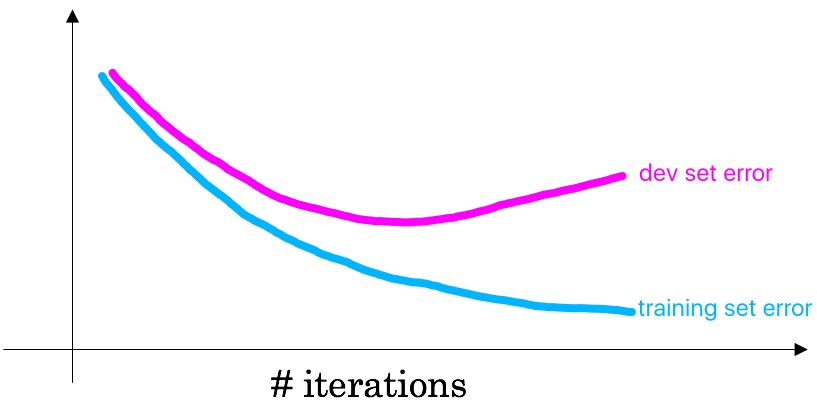
\includegraphics[width=40em]{figures/early-stopping}
    \caption{Early stopping}
    \label{fig:early-stopping}
\end{figure}

Why dose this work? When you haven't run many iterations for your neural networks yet, your
parameters $\Matrix{W}$ will be close to zero, because with random initialization you
probably initialize $\Matrix{W}$ to small random values. And as you iterate, as you train,
$\Matrix{W}$ will get bigger and bigger until you end, then you have a larger $\Matrix{W}$ at last.
So what early stopping does is, by stopping halfway, you have only a mid-size rate $\Matrix{W}$.
And so similar to $L_2$ regularization by picking a neural network with smaller norm for your
parameters $\Matrix{W}$, hopefully your neural network is overfitting less.

We can think of machine learning process as comprising several different steps:
\begin{enumerate}
    \item Optimize cost function $J$. (Gradient descent, etc.)
    \label{step:machine-learning-step-one}
    \item Not overfitting. (Regularization, dropout, etc.)
    \label{step:machine-learning-step-two}
\end{enumerate}

When we have a set of tools for optimizing the cost function $J$, and when you are focusing on
optimizing the cost function $J$, all you care about is finding $\Matrix{W}$ and $\Vector{b}$, so
that $J(\Matrix{W}, \Vector{b})$ is as small as possible. You just don't think about anything else
than Step~\ref{step:machine-learning-step-one}. Then it's completely separate task to not
overfit, in other words, to reduce variance. And when you're doing that, you have a separate set of
tools for doing it. This principle is sometimes called orthogonalization.

The main downside of early stopping is that it couples the above two tasks, so you no longer can
work on these two problems independently. Becaues by stopping gradient descent early, you're sort
of breaking whatever you're doing to optimize cost function $J$. That means when you are optimizing
cost function $J$, you are trying to not overfit simultaneously. So instead of using different
tools to solve the two problems, you are using one that kind of mixes the two, and this just makes
the set of things you could try more complicated to think about.

Rather than using early stopping, one alternative is just use $L_2$ regularization, then you can
just train the neural network as long as possible. You can find this makes the search space of
hyperparameters easier to decompose and easier to search over. But the downsid of this though is
that you might have to try a lot of values of the regularization parameter $\lambda$, which is more
computationally expensive.

The advantage of early stopping is that running the gradient descent process just once, you get to
try out values of small $\Matrix{W}$, mid-size $\Matrix{W}$ and large $\Matrix{W}$, without needing
to try a lot of values of the $L_2$ regularization hyperparameter $\lambda$.

\subsection{Setting up your optimization problem}
\subsubsection{Normalizing inputs}
\paragraph{Normalizing training sets}

When training a neural network, one of the techniques that will speed up your training is if you
normalize your inputs.

Normalizing your inputs correspondes to two steps:
\begin{enumerate}
    \item Subtract out (zero out) the mean
    $$ \mu = \frac{1}{m} \sum_{i=1}^m x^{(i)} $$
    $$ x := x - \mu $$
    \item Normalize the variances
    $$ \sigma = \frac{1}{m} \sum_{i=1}^m {x^{(i)}}^2 \quad \text{(element-wise square)}$$
    $$ x :=  x / \sigma^2 $$
\end{enumerate}

Use the same $\mu$ and $\sigma^2$ to normalize test sets.

\paragraph{Why normalize inputs?}

\begin{figure}[htb]
    \centering
    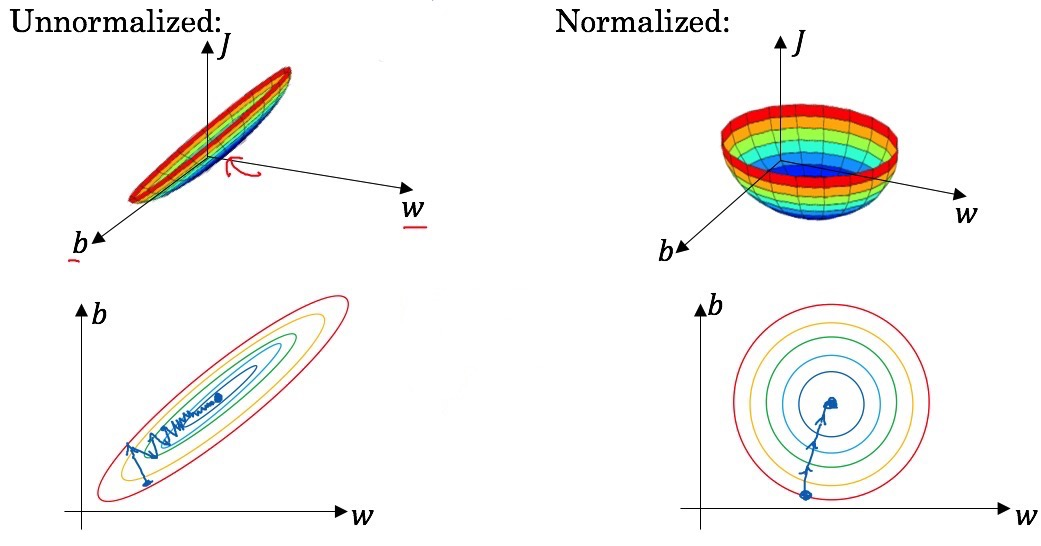
\includegraphics[width=40em]{figures/normalization}
    \caption{Unnormalized features vs. Normalized features}
    \label{fig:normalization}
\end{figure}

Recall the cost function $J$:
$$ J(\Matrix{W}, \Vector{b}) = \frac{1}{m} \sum_{i=1}^m \Cal{L}(\hat{y}^{(i)}, y^{(i)}) $$

If you use unnormalized input features, it's more likely your cost function will look like the left
one in Figure~\ref{fig:normalization}. And if you're running gradient descent on the cost function
like the one on the left, then you might have to use a very small learning rate. Whereas if you
have a more spherical contours, then wherever you start, gradient descent can pretty much go
straight to the minimum. You can take much larger steps with gradient descent rather needing to
oscillate around like the picture on the left.

Of course in practice $W$ is a high-dimensional vector and so try to plot this in 2D doesn't convey
all the intuitions correctly. But the rough intuition that your cost function will be more round
and easier to optimize when your features are all on similar scales.

\subsubsection{Vanishing/Exploding gradients}
One of the problems of training a neural network, especially very deep neural networks, is that
vanishing and exploding gradients. What that means is that when you're training a very deep network
your derivatives or your slopes can sometimes get either very big or very small, maybe even
exponentially small and this makes training difficult.

\begin{figure}[htb]
    \centering
    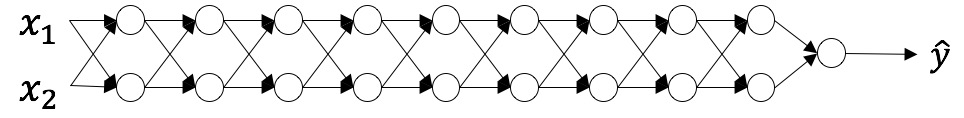
\includegraphics[width=40em]{figures/vanishing-exploding-gradients}
    \caption{Vanishing/explosing gradients}
    \label{fig:vanishing-exploding-gradients}
\end{figure}

In Figure~\ref{fig:vanishing-exploding-gradients}, there is a deep neural network with only two
units in each hidden layer. We have $\Matrix{W}^{[1]}, \Matrix{W}^{[2]}, \ldots, \Matrix{W}^{[L]}$
parameters in this example, and we set $g^{[l]}(z) = z$, which means a linear activation function,
and with $\Vector{b}^{[l]} = 0$. Then the output $\hat{y}$ can be calculated as following:
\begin{IEEEeqnarray*}{rCl}
    \hat{y} = \Matrix{W}^{[L]} \Matrix{W}^{[L-1]} \cdots \Matrix{W}^{[2]} \Matrix{W}^{[1]}
    \Vector{x}
\end{IEEEeqnarray*}

Now, let's say that each of your weight matrices
$\Matrix{W}^{[l]} = \left[\begin{array}{cc} 1.5 & 0 \\ 0 & 1.5 \end{array}\right]$
(excluded $\Matrix{W}^{[L]}$), then
$\hat{y} = \Matrix{W}^{[L]} \left[\begin{array}{cc} 1.5 & 0 \\ 0 & 1.5 \end{array}\right]^{L-1}
\Vector{x}$, so $\hat{y}$ will be like $1.5^{L-1} \Vector{x}$. If $L$ is very large, $\hat{y}$ will
be exploded.

Conversely, If we replace 1.5 with 0.5, which is less than 1, then $\hat{y}$ becomes to
$0.5^{L-1} \Vector{x}$. So if $L$ is large, the activation values will decrease exponentially.

To conclude, with a very deep network, if $\Matrix{W}^{[l]} > I$, then the activations can explode;
and if $\Matrix{W}^{[l]} < I$, then the activations may decrease exponentially. Similarly, the
derivatives or the gradients will also increase exponentially or decrease exponentially.

\subsubsection{Weights Initialization for Deep Networks}
A partial solution to vanishing/exploding of deep networks is more careful choice of the random
initialization of your neural network. To understand this, let's start with the example of
initializing the weights for a single neuron in
Figure~\ref{fig:random-initialization-for-single-neuron}, and then we're going to generalize this
to a deep network.

\begin{figure}[htb]
    \centering
    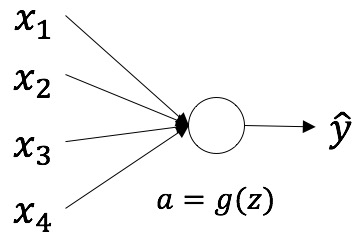
\includegraphics[width=20em]{figures/random-initialization-for-single-neuron}
    \caption{Random initialization for single neuron}
    \label{fig:random-initialization-for-single-neuron}
\end{figure}

We can get
$$ z = w_1 x_1 + w_2 x_2 + \cdots + w_n x_n \quad \text{(ignore b here)} $$
With a large $n$, in order to make $z$ not blow up and not become too small, we need a smaller
$w_i$ for each adding item. One reasonable thing to do would be to set the variance of $w_i$ to be
equal to $\frac{1}{n}$, i.e.
$$ \text{Var}(w:) = \frac{1}{n} $$
where $n$ is the number of input features that's going into a neuron. So in
practice, what you can do is set the weight matrix $\Matrix{W}$ for a certain layer to be
$$\Matrix{W}^{[l]} = \text{np.random.randn(shape)} * \text{np.sqrt(} \frac{1}{n^{[l-1]}} \text{)}$$

It turns out that if you are using a ReLU activation function $g^{[l]} = \text{ReLU}(z)$, rather
than $\frac{1}{n}$, set the variance $\frac{2}{n}$ works a little better
$$ \text{Var}(w:) = \frac{1}{n} $$
$$\Matrix{W}^{[l]} = \text{np.random.randn(shape)} * \text{np.sqrt(} \frac{2}{n^{[l-1]}} \text{)}$$

For more general case, if the input features of actvations are roughly mean 0 and standard variance
1 then this would cause $z$ to also take on a similar scale. This doesn't solve the
vanishing/exploding problem, but it definitely reduce the problem. Because it's trying to set
$\Matrix{W}^{[l]}$ not too much bigger than 1 and not too much less than 1, so it doesn't explode
or vanish too quickly.

\paragraph{Other variaces}
For tanh activation function,
$$ \Matrix{W}^{[l]} = \text{np.random.randn(shape)} * \text{np.sqrt(} \frac{1}{n^{[l-1]}} \text{)}
\quad \text{(Xavier Initialization)} $$
or
$$ \Matrix{W}^{[l]} = \text{np.random.randn(shape)} * \text{np.sqrt(} \frac{2}{n^{[l-1]} + n^{[l]}}
\text{)} \quad \text{(Yoshua Bengio)} $$

In practice, all these formulas just give you a starting point, it gives you a default value to use
for the variance of the initialization of your weight matrices. If you wish the variace in the
formula, this variance parameter could be another thing that you could tune of your hyperparameters.

\subsubsection{Numerical approximation of gradients}
When you implement backpropagation you'll find that there's a test called gradient checking that
can really help you make sure that your implementation of backpropagation is correct.

\paragraph{Checking your derivative computation}

\begin{figure}[htb]
    \centering
    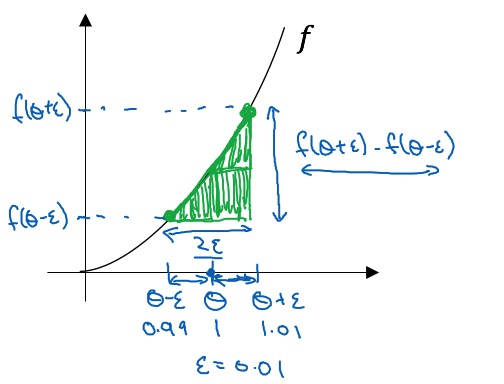
\includegraphics[width=20em]{figures/checking-derivatives}
    \caption{Derivative approximation}
    \label{fig:checking-derivatives}
\end{figure}

We can use two sided difference to estimate the derivatives:
$$ g(\theta) \approx \frac{f(\theta + \epsilon) - f(\theta - \epsilon)}{2 \epsilon} $$

For example, $f(\theta) = \theta^3$ in Figure~\ref{fig:checking-derivatives}, then we can estimate
the derivative at $\theta = 1$ with $\epsilon = 0.01$:
$$ g(1) \approx \frac{(1.01)^3 - (0.99)^3}{2 * 0.01} = 3.0001 $$

And the real deivative at $\theta = 1$ is
$$ g(1) = 3 \theta^2|_{\theta=1} = 3 $$

So the approximation error is 0.0001 ($O(\epsilon^2)$). If we only consider the one side difference
(in range $(\theta, \theta+\epsilon)$), so error will be 0.03 ($O(\epsilon)$). So two sided
difference have more confident approximation than one side difference, it's more accurate, but it
runs twice as slow as it.

\subsubsection{Gradient checking}
Gradient checking can be used to debug and verify your implementation of backpropagation.

Take $\Matrix{W^{[1]}}, \Vector{b^{[1]}}, \ldots, \Matrix{W^{[L]}}, \Vector{b^{[L]}}$ and reshape
into a big vector $\Vector{\theta}$. Then
$$ J(\Vector{\theta}) = J(\Vector{\theta}_1, \Vector{\theta}_2, \ldots)
= J(\Matrix{W^{[1]}}, \Vector{b^{[1]}}, \ldots, \Matrix{W^{[L]}}, \Vector{b^{[L]}}) $$

Take $\text{d}\Matrix{W^{[1]}}, \text{d}\Vector{b^{[1]}}, \ldots, \text{d}\Matrix{W^{[L]}},
\text{d}\Vector{b^{[L]}}$ and reshape into a big vector $\text{d}\Vector{\theta}$. Now we have a
question, is $\text{d}\Vector{\theta}$ the gradient or the slope of $J(\Vector{\theta})$?

\begin{algorithm}[htb]
\For{each $i$}{
    d$\displaystyle \Vector{\theta}_{approx}[i]
    = \frac{J(\Vector{\theta}_1, \Vector{\theta}_2, \ldots, \Vector{\theta}_i + \epsilon, \ldots)
     - J(\Vector{\theta}_1, \Vector{\theta}_2, \ldots, \Vector{\theta}_i-\epsilon, \ldots)}
     {2 \epsilon}$
}
\end{algorithm}

We have known that $\displaystyle \text{d}\Vector{\theta}_{approx}[i]
\approx \text{d}\Vector{\theta}[i] = \frac{\partial J}{\partial \Vector{\theta}_i}$.

Let $\epsilon = 10^{-7}$, then we check the value of
$$ \frac{||\text{d}\Vector{\theta}_{approx} - \text{d}\Vector{\theta}||_2}
{||\text{d}\Vector{\theta}_{approx}||_2 + ||\text{d}\Vector{\theta}||_2} $$

If the value is close to $\epsilon$, then that's great, it means your derivative approximation is
very likely correct. If it's maybe on the then range around $10^{-5}$, you should be careful and
double-check the components of the vector. And if the value is about $10^{-3}$, then it's more
concerned that there's a bug somewhere.

\subsubsection{Gradient Checking Implementation Notes}
\begin{itemize}
    \item Don't use in training - only to debug
    \item If algorithm fails grad check, look at componets (where are different) to try to identify
    bug
    \item Remember regularization
    \item Doesn't work with dropout
    \item Run at random initialization; perhaps again after some training
\end{itemize}

\section{Optimization algorithms}

\subsection{Optimization algorithms}
Optimization algorithms can enable us to train our neural network much faster. Applying machine
learning is a highly empirical process, is a highly iterative process. One thing that makes it
more difficult is that Deep Learning does not work best in a regime of big data, we are able to
train neural networks on a large data set, and training on a huge data set is just slow. Having
good and fast optimization algorithms can really speed up the efficiency of you and your team.

\subsubsection{Mini-batch gradient descent}
\paragraph{Batch vs. mini-batch gradient descent}
Vectorization allows you to efficiently compute on $m$ examples:
$$ \Matrix{X} = \left[\begin{array}{cccc} \Vector{x^{(1)}} & \Vector{x^{(2)}} & \cdots
& \Vector{x^{(m)}}\end{array}\right] \qquad \Matrix{X} \in \Set{R}^{(n_x, m)} $$
$$ \Matrix{Y} = \left[\begin{array}{cccc} \Vector{y^{(1)}} & \Vector{y^{(2)}} & \cdots
& \Vector{y^{(m)}}\end{array}\right] \qquad \Matrix{Y} \in \Set{R}^{(1, m)} $$

If $m$ is very large (say 5 million), then training can be very slow. With the implementation of
gradient descent on your whole training set, what you have to do is you have to process your entire
training set before you take one little step of gradient descent. So it turns out you can get a
faster algorithm if you let gradient descent start to make some progress even before you finish
processing your entire your giant training sets.

Let's say you split up your training set into little baby training sets and these baby training
sets are called mini-batches, and use $\Matrix{X^{\{t\}}}$ and $\Matrix{Y^{\{t\}}}$ to denote them.
Every mini-batch contains 1000 examples, there are 5000 mini-batches in total.
$$ \Matrix{X} = \left[\begin{array}{ccccc} \Matrix{X^{\{1\}}} & \Matrix{X^{\{2\}}} & \cdots
& \Matrix{X^{\{t\}}} & \cdots \end{array}\right] $$
$$ \Matrix{Y} = \left[\begin{array}{ccccc} \Matrix{Y^{\{1\}}} & \Matrix{Y^{\{2\}}} & \cdots
& \Matrix{Y^{\{t\}}} & \cdots \end{array}\right] $$

\paragraph{Mini-batch gradient descent}

\begin{algorithm}[htb]
\tcp{Mini-batch gradient descent algorithm}
\Repeat{converge}{
    \tcp{5000 mini-batches}
    \For{t = 1, 2, \ldots, 5000}{
        \For{prop on $\Matrix{X^{\{t\}}}$}{
            $\displaystyle \Matrix{Z^{[1]}} = \Matrix{W^{[1]}} \Matrix{X^{\{t\}}}
                + \Vector{b^{[1]}}$ \\
            $\displaystyle \Matrix{A^{[1]}} = g^{[1]}(\Matrix{Z^{[1]}})$ \\
            \ldots \\
            $\displaystyle \Matrix{Z^{[l]}} = \Matrix{W^{[1]}} \Matrix{X^{\{t\}}}
                + \Vector{b^{[l]}}$ \\
            $\displaystyle \Matrix{A^{[l]}} = g^{[l]}(\Matrix{Z^{[l]}})$
        }
        \tcp{Compute cost J, 1000 examples in each mini-batch (the size of the mini-batch)}
        $\displaystyle J^{\{t\}} = \frac{1}{1000} \sum_{i=1}^{l}\Cal{L}
        \underbrace{(\hat{y^{(i)}}, y^{(i)})}_{\text{from } \Matrix{X^{\{t\}}}, \Matrix{Y^{\{t\}}}}
        + \frac{\lambda}{1000}$ \\
        \tcp{Backprop to compute gradients w.r.t. $J^{\{t\}}$
        (using $\Matrix{X^{\{t\}}}, \Matrix{Y^{\{t\}}}$)}
        $\Matrix{W^{[l]}} := \Matrix{W^{[l]}} - \alpha \text{d}\Matrix{W^{[l]}}, \quad
        \Vector{b^{[l]}} := \Vector{b^{[l]}} - \alpha \text{d}\Vector{b^{[l]}}$
    }
}
\end{algorithm}

With mini-batch gradient descent, a single pass through the training set, that is one epoch, allows
you to take 5000 gradient steps.

\subsubsection{Understanding mini-batch gradient descent}
With batch gradient descent, on every iteration you go through the entire training set, you'd
expect the cost to go down on every single iteration. On mini-batch gradient descent though, if you
plot progress on your cost function, then it may not decrease on every iteration.

In paricular, on every iteration, you are processing some $\Matrix{X^{\{t\}}}, \Matrix{Y^{\{t\}}}$
and so if you plot the cost function $J^{\{t\}}$, which is computed using just
$\Matrix{X^{\{t\}}}, \Matrix{Y^{\{t\}}}$, then it's as if on every iteration you're training on a
different training dataset or really training on a different mini-batch. So you plot the cost
function $J^{\{t\}}$, it should trend downwards, but it's also going to be a little bit noiser,
which can be seen in Figure~\ref{fig:training-mini-batch}.

\begin{figure}[htb]
    \centering
    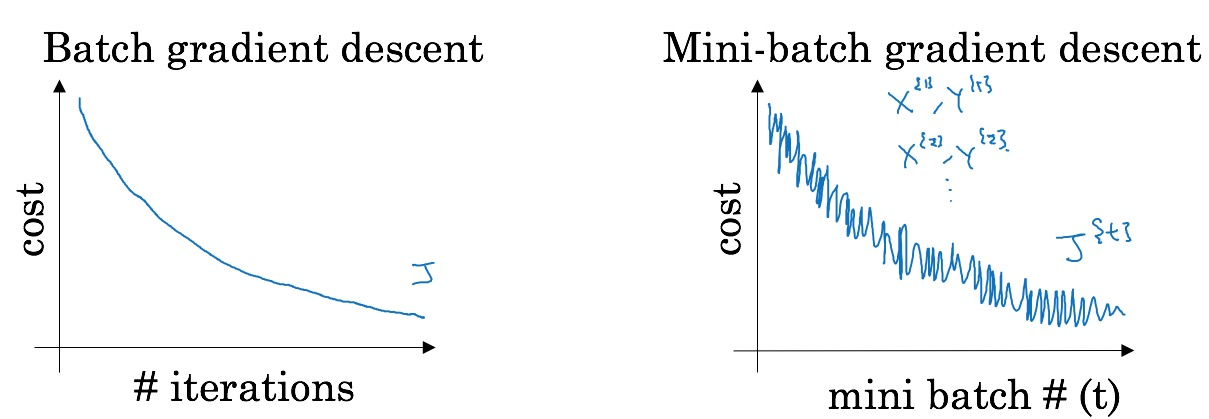
\includegraphics[width=40em]{figures/training-mini-batch}
    \caption{Training with mini-batch gradient descent}
    \label{fig:training-mini-batch}
\end{figure}

\paragraph{Choosing your mini-batch size}
$$\begin{array}{lll}
    \text{If mini-batch size} = $m$: & \text{Batch Gradient Descent} &
    (\Matrix{X^{\{t\}}}, \Matrix{Y^{\{t\}}}) = (\Matrix{X}, \Matrix{Y}). \\
    \text{If mini-batch size} = $1$: & \text{Stochastic Gradient Descent} &
    \text{Each example is its own mini-batch } (t = i)
\end{array}$$

The batch gradient descent might start somewhere and be able to take relatively low noise,
relatively large steps, just keep matching to minimum. In contrast with stochastic gradient descent,
if you start somewhere, then on every iteration you're taking gradient descent with just a signle
training example, so most of the time you head toward the global optimum, but sometimes you head to
the wrong direction if that one example happens to point you in a bad direction. So stochastic
gradient can be extremly noisy. On average, it'll take you in a good direction, but sometimes it'll
head in the wrong direction as well. As stochastic gradient descent won't ever converge, it will
always just kind of oscillate and wander around the region of the minimum, which can be seen in
Figure~\ref{fig:choosing-mini-batch-size}.

\begin{figure}[htb]
    \centering
    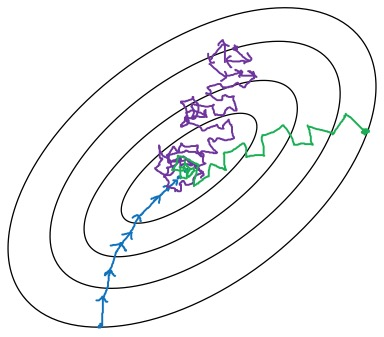
\includegraphics[width=20em]{figures/choosing-mini-batch-size}
    \caption{Choose mini-batch size. If the size is $m$, it's Batch Gradient Descent; If the size
    is 1, it's Stochastic Gradient Descent; If the size is between 1 and $m$, it's Mini-batch
    Gradient Descent.}
    \label{fig:choosing-mini-batch-size}
\end{figure}

\subsubsection{Exponentially wighted averages}

Figure~\ref{fig:temperature-in-london} shows the temperature in London for a year. The data (blue
points) looks a little noisy, we want to compute the trends of the local average of the temperature.
Then we can use $v_i$ to denote the temperature in $i$-th day, and
$$v_0 = 0$$
$$v_1 = 0.9v_0 + 0.1\theta_1$$
$$v_2 = 0.9v_1 + 0.1\theta_2$$
$$\vdots$$
$$v_t = 0.9v_{t-1} + 0.1\theta_t$$

We can think $v_t$ as approximately averaging over $\displaystyle \frac{1}{1-\beta}$ days'
temperature.

$$ v_t = \beta v_{t-1} + (1-\beta)\theta_t $$

\begin{itemize}
    \item $\beta = 0.9$: $approx$ 10 days' temperature
    \item $\beta = 0.98$: $approx$ 50 day's temperature
    \item $\beta = 0.5$: $approx$ 2 day's temperature
\end{itemize}

\begin{figure}[htb]
    \centering
    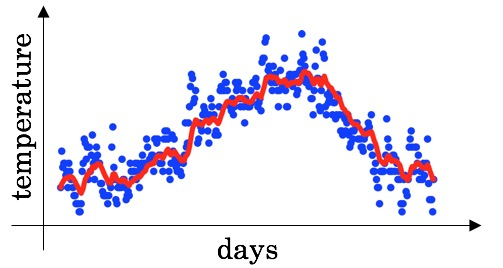
\includegraphics[width=20em]{figures/temperature-in-london-1}
    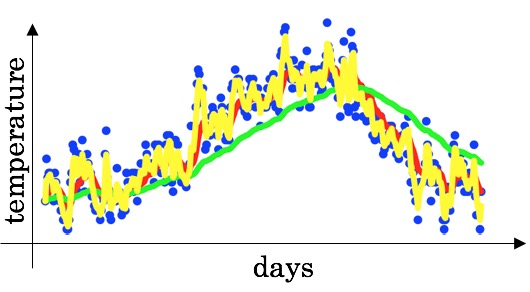
\includegraphics[width=20em]{figures/temperature-in-london-2}
    \caption{Temperature in London for one year. $\beta = 0.9$ for red line; $\beta = 0.98$ for
    green line; $\beta = 0.5$ for yellow line.}
    \label{fig:temperature-in-london}
\end{figure}

\subsubsection{Understanding exponetially weighted averages}
$$ v_t = \beta v_{t-1} + (1-\beta)\theta_t $$

$$ v_{100} = 0.9 v_{99} + 0.1\theta_{100} $$
$$ v_{99} = 0.9 v_{98} + 0.1\theta_{99} $$
$$ v_{98} = 0.9 v_{97} + 0.1\theta_{98} $$
$$ \ldots $$

\begin{IEEEeqnarray*}{rCl}
    v_{100} = 0.1\theta_{100} + 0.9v_{99} = 0.1 \theta_{100} + 0.1 \times 0.9 \theta_{99}
    + 0.1 (0.9)^2 \theta_{98} + 0.1 (0.9)^3 \theta_{97} + \cdots
\end{IEEEeqnarray*}

\begin{figure}[htb]
    \centering
    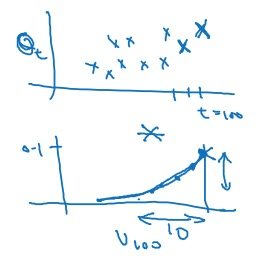
\includegraphics[width=25em]{figures/exp-weighted-average}
    \caption{The $v_{100}$ can be seen as the element-wise multiplication of $\theta_t$ and the
    exponentially distribution.}
    \label{fig:exp-weighted-average}
\end{figure}

$$ (1 - \epsilon)^{\frac{1}{\epsilon}} = \frac{1}{e} \approx 0.35 $$
The hight of $\displaystyle \frac{1}{e}$ in the exponentially distribution in
Figure~\ref{fig:exp-weighted-average} is respect to $\displaystyle \frac{1}{\epsilon}$ days on the
horizontal axis.

\begin{algorithm}[htb]
    \tcp{Implementing exponetially weighted averages}
    $v_{\theta} = 0$ \\
    \Repeat{t = maxDays}{
        Get next $\theta_t$ \\
        $v_{\theta} := \beta v_{\theta} + (1-\beta) \theta_t$
    }
\end{algorithm}

\subsubsection{Bias correction in exponentially weighted averages}
When $t$ is small, there is a bias because we take $v_0 = 0$, we can correct that in the following
way.

$$ v_t = \beta v_{t-1} + (1-\beta)\theta_t $$

$$ v_t := \frac{v_t}{1 - \beta^t} $$

\subsubsection{Gradient descent with momentum}

Because mini-batch gradient descent makes a parameter update after seeing just a subset of example,
the direction of the update has some variance, and so the path taken by mini-batch gradient descent
will ``oscillate'' toward convergence, like Figure~\ref{fig:momentum}. Using momentum can reduce
these oscillations.

Momentum takes into account the past gradients to smooth out the update. We will store the
`direction' of the previous gradient in the variable $v$. Formally, this will be the exponentially
weighted average of the gradient on previous steps. You can also think of $v$ as the ``velocity''
of a ball rolling downhill, building up speed (and momentum) according to the direction of the
gradient/slope of the hill.

\begin{figure}[htb]
    \centering
    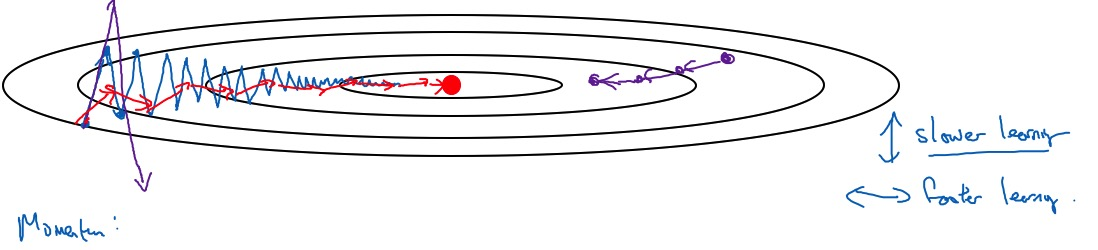
\includegraphics[width=45em]{figures/momentum}
    \caption{Momentum can reduce the oscillation and sooth out the update.}
    \label{fig:momentum}
\end{figure}

\begin{algorithm}[htb]
    \tcp{Momentum optimization algorithm}
    $\displaystyle v_{\text{d}\Matrix{W}} = \Matrix{0}$,
    $\displaystyle v_{\text{d}\Vector{b}} = \Vector{0}$ \\
    \For{iteration t}{
        Compute d$\Matrix{W}$, d$\Vector{b}$ on current mini-batch. \\
        $\displaystyle v_{\text{d}\Matrix{W}} = \beta v_{\text{d}\Matrix{W}}
        + (1 - \beta)\text{d}\Matrix{W}$ \qquad
        $\displaystyle v_{\text{d}\Vector{b}} = \beta v_{\text{d}\Vector{b}}
        + (1 - \beta)\text{d}\Vector{b}$ \\
        $\displaystyle \Matrix{W} := \Matrix{W} - \alpha v_{\text{d}\Matrix{W}}$ \qquad
        $\displaystyle \Vector{b} := \Vector{b} - \alpha v_{\text{d}\Vector{b}}$
    }
\end{algorithm}

Now we have two hyperparameters $\alpha$ and $\beta$, the most common value for $\beta$ is 0.9.

In practice, people usually don't do bias correction when implementing gradient descent or momentum.
Because after just ten iterations your moving average will have warmed up and is no longer a bias
estimate.

\subsubsection{RMSprop}
RMSprop (Root Mean Square prop) can also speed up gradient descent.

\begin{algorithm}[htb]
    \tcp{RMSprop optimization algorithm}
    $\displaystyle s_{\text{d}\Matrix{W}} = \Matrix{0}$,
    $\displaystyle s_{\text{d}\Vector{b}} = \Vector{0}$ \\
    \For{iteration t}{
        Compute d$\Matrix{W}$, d$\Vector{b}$ on current mini-batch. \\
        $\displaystyle s_{\text{d}\Matrix{W}} = \beta_2 s_{\text{d}\Matrix{W}}
        + (1 - \beta_2){\text{d}\Matrix{W}}^2$ \qquad
        $\displaystyle s_{\text{d}\Vector{b}} = \beta_2 s_{\text{d}\Vector{b}}
        + (1 - \beta_2){\text{d}\Vector{b}}^2$ \\
        $\displaystyle \Matrix{W} := \Matrix{W}
        - \alpha \frac{\text{d}\Matrix{W}}{\sqrt{s_{\text{d}\Matrix{W}}} + \epsilon}$ \qquad
        $\displaystyle \Vector{b} := \Vector{b}
        - \alpha \frac{\text{d}\Matrix{b}}{\sqrt{s_{\text{d}\Matrix{b}}} + \epsilon}$
    }
\end{algorithm}

$\epsilon = 10^{-8}$ is reasonable default to ensure numberical stability.

\subsubsection{Adam optimization algorithm}
\begin{algorithm}[htb]
    \tcp{Adam optimization algorithm}
    $\displaystyle v_{\text{d}\Matrix{W}} = \Matrix{0}$,
    $\displaystyle s_{\text{d}\Matrix{W}} = \Matrix{0}$,
    $\displaystyle v_{\text{d}\Vector{b}} = \Vector{0}$,
    $\displaystyle s_{\text{d}\Vector{b}} = \Vector{0}$ \\
    \For{iteration t}{
        Compute d$\Matrix{W}$, d$\Vector{b}$ on current mini-batch. \\
        $\displaystyle v_{\text{d}\Matrix{W}} = \beta_1 v_{\text{d}\Matrix{W}}
        + (1 - \beta_1)\text{d}\Matrix{W}$ \qquad
        $\displaystyle v_{\text{d}\Vector{b}} = \beta_1 v_{\text{d}\Vector{b}}
        + (1 - \beta_1)\text{d}\Vector{b}$ \\
        $\displaystyle s_{\text{d}\Matrix{W}} = \beta_2 s_{\text{d}\Matrix{W}}
        + (1 - \beta_2){\text{d}\Matrix{W}}^2$ \qquad
        $\displaystyle s_{\text{d}\Vector{b}} = \beta_2 s_{\text{d}\Vector{b}}
        + (1 - \beta_2){\text{d}\Vector{b}}^2$ \\
        $\displaystyle v_{\text{d}\Matrix{W}}^{\text{corrected}}
        = \frac{v_{\text{d}\Matrix{W}}}{1 - \beta_1^t}$ \qquad
        $\displaystyle v_{\text{d}\Matrix{b}}^{\text{corrected}}
        = \frac{v_{\text{d}\Matrix{b}}}{1 - \beta_1^t}$ \\
        $\displaystyle s_{\text{d}\Matrix{W}}^{\text{corrected}}
        = \frac{s_{\text{d}\Matrix{W}}}{1 - \beta_2^t}$ \qquad
        $\displaystyle s_{\text{d}\Matrix{b}}^{\text{corrected}}
        = \frac{s_{\text{d}\Matrix{b}}}{1 - \beta_2^t}$ \\
        $\displaystyle \Matrix{W} := \Matrix{W}
        - \alpha \frac{\text{d}\Matrix{W}}{\sqrt{s_{\text{d}\Matrix{W}}} + \epsilon}$ \qquad
        $\displaystyle \Vector{b} := \Vector{b}
        - \alpha \frac{\text{d}\Matrix{b}}{\sqrt{s_{\text{d}\Matrix{b}}} + \epsilon}$
    }
\end{algorithm}

\paragraph{Hyperparameters choice}
\begin{itemize}
    \item $\alpha$: needs to be tune
    \item $\beta_1$: 0.9 ($\text{d}\Matrix{W}$)
    \item $\beta_2$: 0.999 (${\text{d}\Matrix{W}}^2$)
    \item $\epsilon$: $10^{-8}$
\end{itemize}

\subsubsection{Learning rate decay}
Learning rate decay can slowly reduce your learning rate over time, which can be seen in
Figure~\ref{fig:learning-rate-decay}.

\begin{figure}[htb]
    \centering
    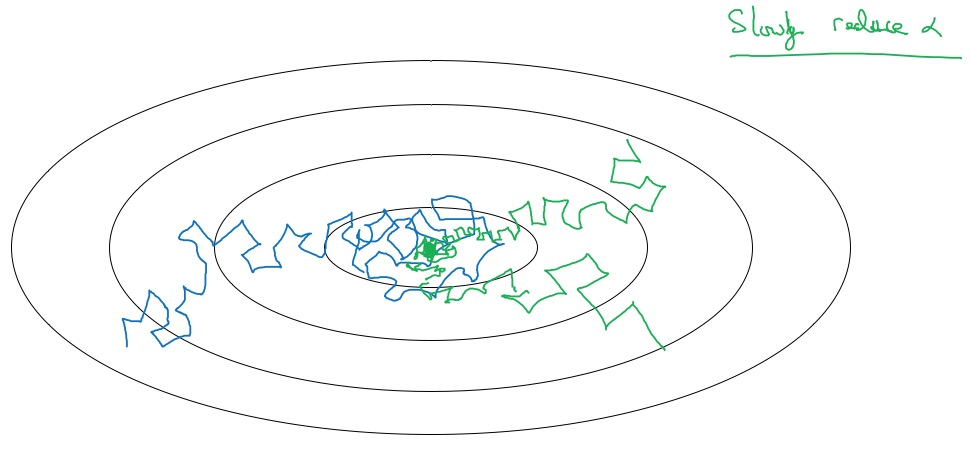
\includegraphics[width=35em]{figures/learning-rate-decay}
    \caption{Learning rate decay}
    \label{fig:learning-rate-decay}
\end{figure}

\begin{algorithm}[htb]
    \tcp{Learning rate decay}
    \For{each epoch (each pass through of data)}{
        $\displaystyle \alpha = \frac{1}{1 + decay_rate * epoch_num} \alpha_0$
    }
\end{algorithm}

\paragraph{Other learning rate decay methods}
\begin{itemize}
    \item $\displaystyle \alpha = 0.95^{epoch_num} \alpha_0$ (exponentially decay)
    \item $\displaystyle \alpha = \frac{k}{\sqrt{epoch_num}} \alpha_0$ \quad or \quad
    $\displaystyle \alpha = \frac{k}{\sqrt{t}} \alpha_0$ \qquad (k is constant)
\end{itemize}

\subsubsection{Local optima in neural networks}
In the early days of deep learning, people used to worry a lot about the optimization algorithm
getting stuck in bad local optima. But as the theory of deep learning has advanced, our
understanding of local optima is also changing.

Figure~\ref{fig:local-optima-1} is what used to have in mind when they worried about local optima,
but this intuition is not always right. It turns out that if you create a neural network, most
points of zero gradients are not local optima, instead most points of zero gradient in a cost
function are saddle points, like Figure~\ref{fig:local-optima-2} shows.

For high dimensional space, it's more likely to run into the local optima instead of a local optima.

\begin{figure}[htb]
    \centering
    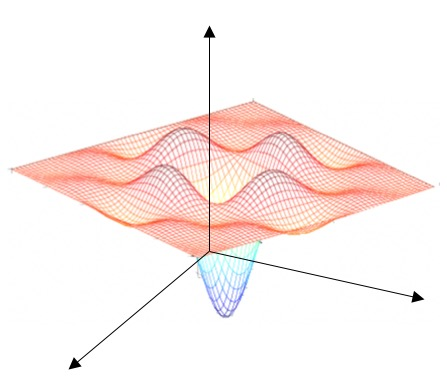
\includegraphics[width=25em]{figures/local-optima-1}
    \caption{The local optima used to be in the mind of people}
    \label{fig:local-optima-1}
\end{figure}

\begin{figure}[htb]
    \centering
    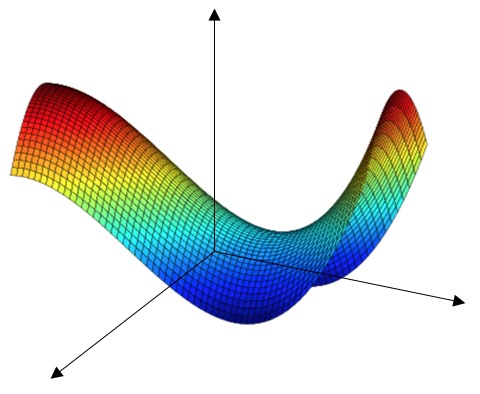
\includegraphics[width=25em]{figures/local-optima-2}
    \caption{What most zero gradient points really look like, saddle points}
    \label{fig:local-optima-2}
\end{figure}

\paragraph{Problem of plateaus}
It turns out that plateaus can really slow down learning and a plateau is region where the
derivatives is close to zero for a long time.

\begin{itemize}
    \item Unlikely to get stuck in a bad local optima
    \item Plateaus can make learning slow
\end{itemize}


\section{Hyperparameter tuning, Batch Normalization and Programming Frameworks}
\subsection{Hyperparameter tuning}
\subsubsection{Tuning process}
The guideline to tune hyperparameters:
\begin{enumerate}
    \item $\alpha$ \quad (Learning rate, the most important hyperparameter)
    \item $\beta$ \quad (Momentum, default 0.9)
    \item mini-batch size
    \item \#hidden units
    \item \#layers
    \item learning rate decay
    \item $\beta_1$, $\beta_2$, $\epsilon$ \quad (Adam, default 0.9/0.999/$10^{-8}$)
\end{enumerate}

\paragraph{Try random values: Don't use a grid}
In earlier generations of machine learning algorithms, grid is okay when the number of
hyperparameters is small. But in deep learning, it's better to sample hyperparameters randomly,
because it's more likely to get a good performance within fewer times.

\paragraph{Coarse to fine}
Like Figure~\ref{fig:coarse-to-fine} shows, you can try some sample points in the hyperparameters
space first, and get some good points. Then zoom in and search in the zoomed region densely. This
is called coarse to fine.

\begin{figure}[htb]
    \centering
    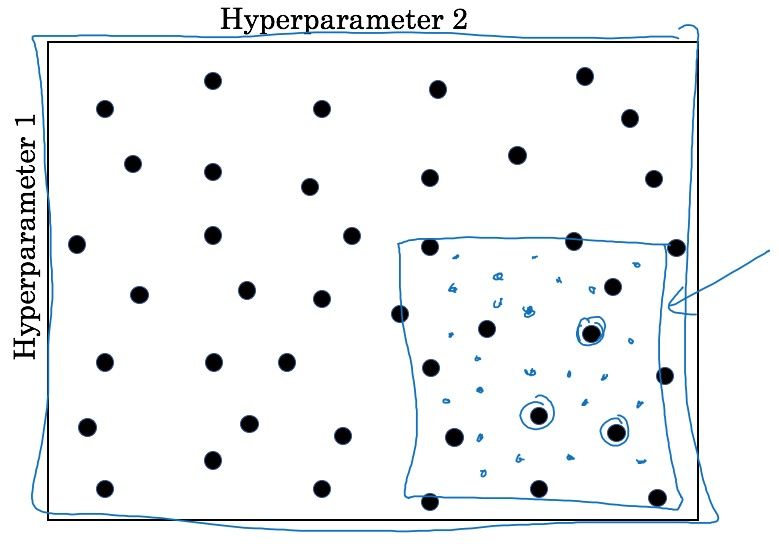
\includegraphics[width=25em]{figures/coarse-to-fine}
    \caption{Coarse to fine}
    \label{fig:coarse-to-fine}
\end{figure}

\subsubsection{Using an appropriate scale to pick hyperparameters}
\paragraph{Appropriate scale for hyperparameters}
For example,
$$\alpha \in [0.0001, 1]$$

Search in a log scale instead of linear scale.

\begin{minted}{numpy}
    r = -4 * np.random.rand() # r ranges in [-4, 0] ([a, b])
    alpha = 10 ** r
\end{minted}

\paragraph{Hyperparameters for exponentially weighted averages}
$$ \beta = [0.9, \ldots, 0.999] $$
$$ 1 - \beta = [0.1, \ldots, 0.001] $$
\begin{minted}{numpy}
    r = -2 * np.random.rand() - 1 # r ranges in [-3, -1] ([a, b])
    beta = 1 - 10 ** r
\end{minted}

Because $\frac{1}{1-\beta}$,
$$ \beta: 0.9000 \rightarrow 0.9005 \quad \text{small impact} $$
$$ \beta: 0.9990 \rightarrow 0.9995 \quad \text{huge impact} $$

\subsubsection{Hyperparameter tuning in Practice: Pandas vs. Caviar}
Figure~\ref{fig:pandas-vs-caviar} shows two ways of tuning hyperparameters.

\begin{figure}[htb]
    \centering
    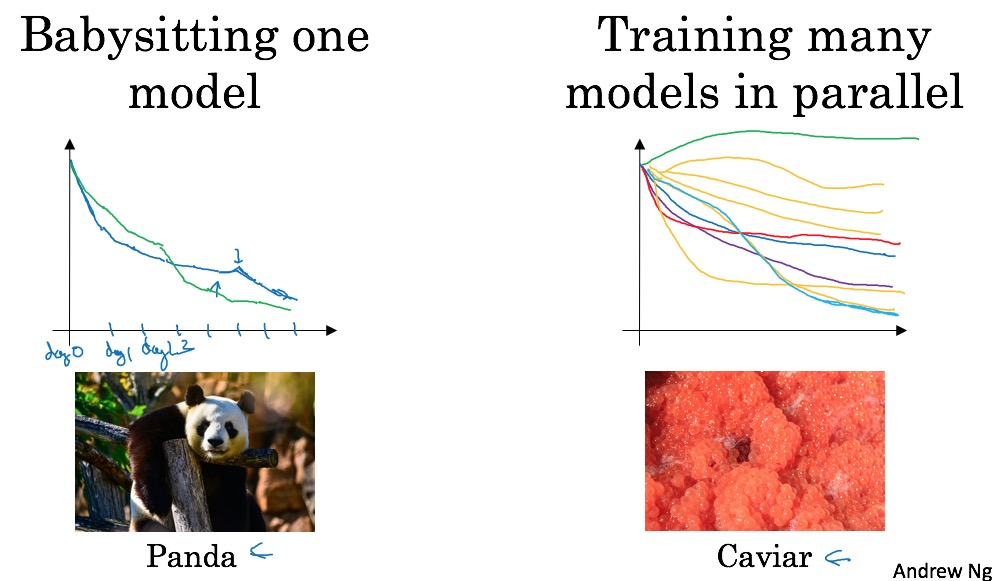
\includegraphics[width=40em]{figures/pandas-vs-caviar}
    \caption{Coarse to fine}
    \label{fig:pandas-vs-caviar}
\end{figure}

\subsection{Batch Normalization}
\subsubsection{Normalization activations in a network}
For example, we can normalize $\Vector{a^{[2]}}$ so as to train $\Matrix{W^{[3]}},
\Vector{b^{[3]}}$ faster, this is called Batch Normalization.
It's more common to do normalization on $\Vector{z^{[2]}}$ instead of $\Vector{a^{[2]}}$.

\begin{algorithm}[htb]
    \tcp{Implementing Batch Norm}
    Given some intermediate values in NN, $\Vector{z^{[l](1)}}, \Vector{z^{[l](2)}}, \ldots,
    \Vector{z^{[l](m)}}$ \\
    $\displaystyle \mu = \frac{1}{m} \sum_{i} \Vector{z^{[l](i)}}$ \\
    $\displaystyle \sigma^2 = \frac{1}{m} \sum_i (\Vector{z^{[l](i)}} - \mu)^2$ \\
    $\displaystyle \Vector{z_{\text{norm}}^{[l](i)}} = \frac{\Vector{z^{[l](i)}}-\mu}
    {\sqrt{\sigma^2 + \epsilon}}$ \\
    $\displaystyle \widetilde{z^{[l](i)}} = \gamma z_{\text{norm}}^{[l](i)} + \beta$ \qquad
    ($\beta$ and $\gamma$ are learnable parameters of the model)
\end{algorithm}

If
$$ \gamma = \sqrt{\sigma^2 + \epsilon} $$
$$ \beta = \mu $$
then
$$ \widetilde{z^{[l](i)}} = z^{[l](i)} $$

Use $\widetilde{z^{[l](i)}}$ instead of $z^{[l](i)}$.

What Batch Norm really does is normalizing in mean and variance of the hidden units values
($z^{[l](i)}$), to have some fixed mean and variance, which are controlled by $\beta$ and $\gamma$.

\subsubsection{Fitting Batch Norm into a neural network}
\begin{figure}[htb]
    \centering
    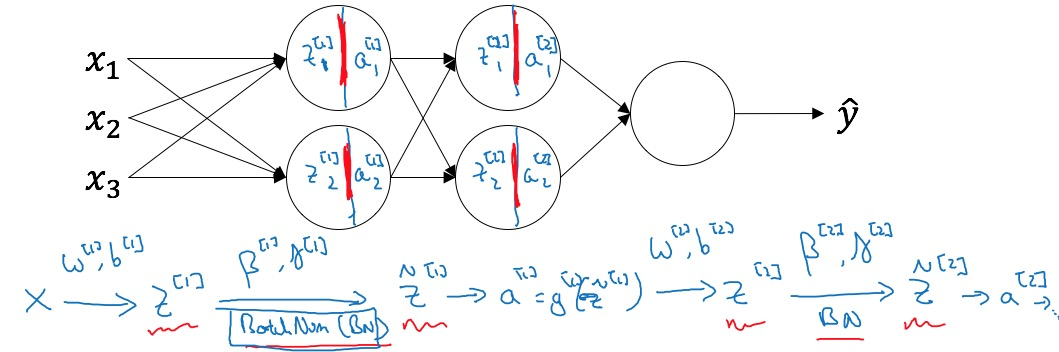
\includegraphics[width=40em]{figures/add-batch-norm-to-a-network}
    \caption{Add Batch Norm to a network}
    \label{fig:add-batch-norm-to-a-network}
\end{figure}

Parameters: $\Matrix{W^{[1]}}$, $\Vector{b^{[1]}}$, $\Matrix{W^{[2]}}$, $\Vector{b^{[2]}}$, \ldots,
$\Matrix{W^{[L]}}$, $\Vector{b^{[L]}}$, \quad
$\beta^{[1]}$, $\gamma^{[1]}$, $\beta^{[2]}$, $\gamma^{[2]}$, \ldots, $\beta^{[L]}$, $\gamma^{[L]}$

Update parameters in the same way:
$$ \beta^{[l]} = \beta^{[l]} - \alpha \text{d}\beta^{[l]} $$

In TensorFlow, we can implement Batch Normalization with
\mintinline{python}{tf.nn.batch_normalization}.

\paragraph{Working with mini-batches}
\begin{figure}[htb]
    \centering
    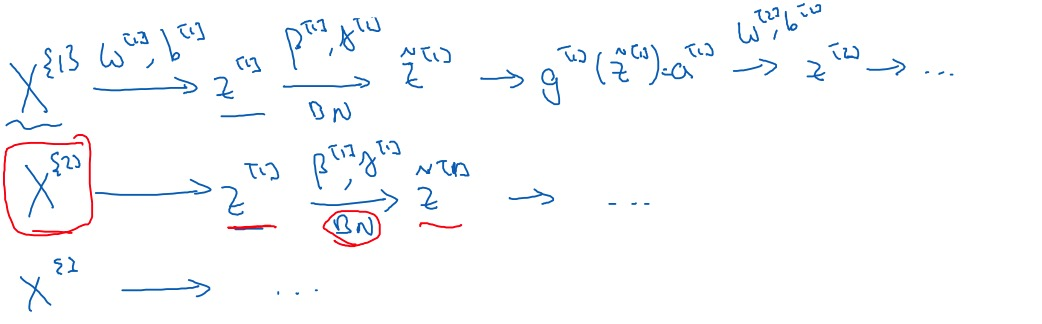
\includegraphics[width=40em]{figures/batch-norm-with-mini-batches}
    \caption{Batch Norm working with mini-batches}
    \label{fig:batch-norm-with-mini-batches}
\end{figure}

Parameters: $\Matrix{W^{[l]}}$, {\color{red} $\Vector{b^{[l]}}$}, $\beta^{[l]}$, $\gamma^{[l]}$.

$$ \Vector{z^{[l]}} = \Matrix{W^{[l]}} \Vector{a^{[l-1]}} + {\color{red} \Vector{b^{[l]}}}
\qquad \longrightarrow \qquad \Vector{z^{[l]}} = \Matrix{W^{[l]}} \Vector{a^{[l-1]}} $$

$$ \widetilde{z^{[l]}} = \gamma^{[l]} z_{\text{norm}}^{[l]} + \beta^{[l]} $$

$\beta^{[l]}$ and $\gamma^{[l]}$ have the same dimension with $b^{[l]}$

\begin{algorithm}[htb]
    \tcp{Implementing gradeint descent with Batch Norm}
    \For{t = 1 $\cdots$ num\_mini\_batches}{
        Compute forward prop on $\Matrix{X^{\{t\}}}$ \\
        In each layer, use Batch Norm to replace $z^{[l]}$ with $\widetilde{z^{[l]}}$. \\
        Use backprop to compute d$\Matrix{W^{[l]}}$, ${\color{red} \text{d}\Vector{b^{[l]}}}$,
        d$\Vector{\beta^{[l]}}$, d$\Vector{\gamma^{[l]}}$ \\
        Update parameters (working with Momentum, RMSprop, Adam etc.)
    }
\end{algorithm}

\subsubsection{Why does Batch Norm work?}
\begin{figure}[htb]
    \centering
    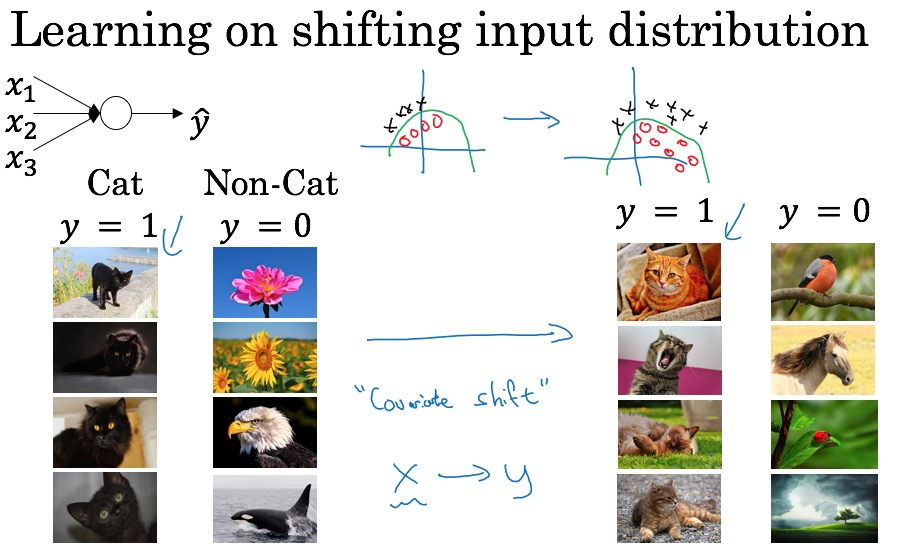
\includegraphics[width=40em]{figures/learning-on-shifting-input-distribution}
    \caption{Batch Norm can help learn on shifting input distribution. Like we learned a netowrk
    which can recognize black cats at first, then we want to use the network to recognize colorful
    cats.}
    \label{fig:learning-on-shifting-input-distribution}
\end{figure}

\begin{figure}[htb]
    \centering
    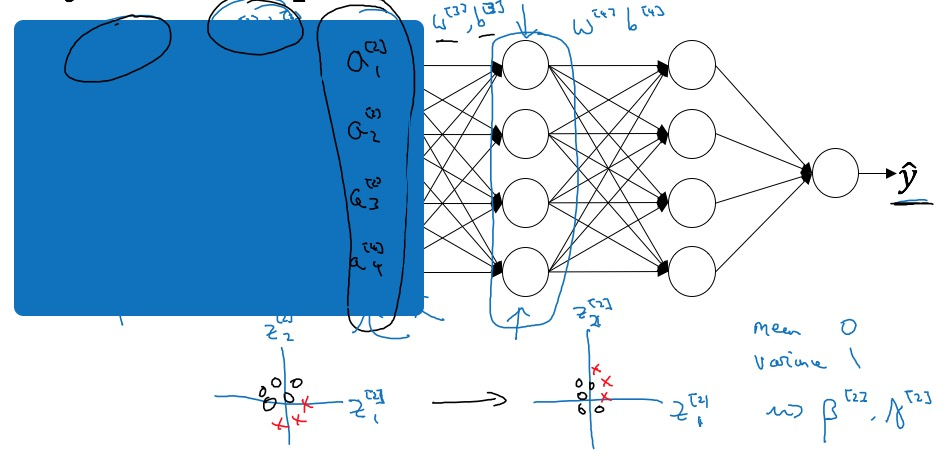
\includegraphics[width=40em]{figures/batch-norm-stable-activations}
    \caption{Batch Norm can stablize the activations in the hidden layers, because of the constains
    of $\beta^{[l]}$ and $\gamma^{[l]}$.}
    \label{fig:batch-norm-stable-activations}
\end{figure}

See Figure~\ref{fig:learning-on-shifting-input-distribution} and
Figure~\ref{fig:batch-norm-stable-activations} for the intuition.

\paragraph{Batch Norm as regularization}
\begin{itemize}
    \item Each mini-batch is scaled by the mean/variance computed on just that mini-batch.
    \item This adds some noise to the values $z^{[l]}$ within that mini-batch. So similar to
    dropout, it adds some noise to each hidden layer's activations.
    \item This has a slight regularization effect. Using lager mini-batch size will reduce this
    effect.
    \item Don't turn to Batch Norm as a regularization.
\end{itemize}

\subsubsection{Batch Norm at test time}
Batch Norm process your data one mini-batch at a time, but at test time you might need to process
the examples one at a time.

When training
$$\displaystyle \mu = \frac{1}{m} \sum_{i} \Vector{z^{[l](i)}}$$
$$\displaystyle \sigma^2 = \frac{1}{m} \sum_i (\Vector{z^{[l](i)}} - \mu)^2$$
$$\displaystyle \Vector{z_{\text{norm}^{[l](i)}}} = \frac{\Vector{z^{[l](i)}}-\mu}
{\sqrt{\sigma^2 + \epsilon}}$$
$$\displaystyle \widetilde{z^{[l](i)}} = \gamma z_{\text{norm}}^{[l](i)} + \beta$$

When testing, using exponentially weighted average (running average) to get estimation of $\mu$ and
$\sigma^2$, then
$$\displaystyle z_{\text{norm}} = \frac{z-\mu}{\sqrt{\sigma^2 + \epsilon}}$$
$$\displaystyle \widetilde{z} = \gamma z_{\text{norm}} + \beta$$

\subsection{Multi-class classification}
\subsubsection{Softmax Regression}
So far, the classfication examples we've talked about have used binary classification, where you
had two possible labels, 0 or 1. There's a generalization of logistic regression called Softmax
regression, which lets you make predictions when you try to recognize one of C or one of the
multiple classes, rather than just recognize just two classes.

$$ \Vector{z^{[L]}} = \Matrix{W^{L}} \Vector{a^{L-1}} + \Vector{b^{[L]}} $$

Activation function:
$$ t = e^{(\Vector{z^{[L]}})} $$
$$ \Vector{a^{L}} = \frac{e^{(\Vector{z^{[L]}})}}{\sum_{j=1}^c t_i}, \quad
\Vector{a_i^{L}} = \frac{t_i}{\sum_{j=1}^c t_i} $$

\begin{figure}[htb]
    \centering
    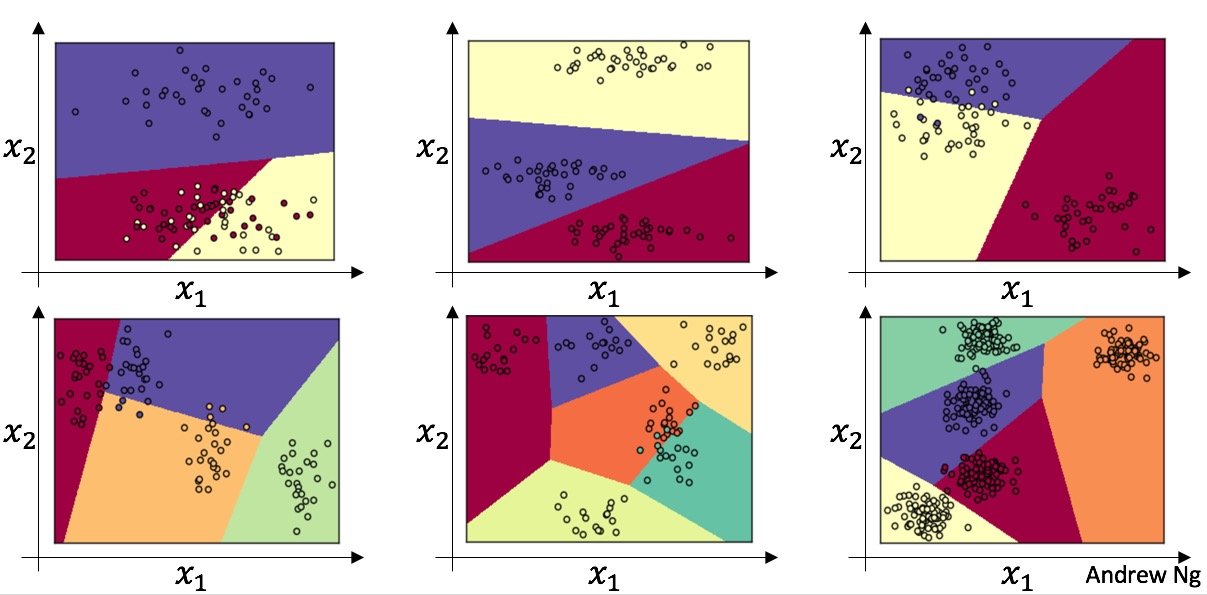
\includegraphics[width=40em]{figures/softmax-examples}
    \caption{Softmax examples, which can be seen as a generalization of logistic regression with
    sort of linear decision boundaries, but with more than two classes.}
    \label{fig:softmax-examples}
\end{figure}

\subsubsection{Training a softmax classifier}
\paragraph{Understanding softmax}
$$ z^{[L]} = \left[\begin{array}{c} 5 \\ 2 \\ -1 \\ 3 \end{array}\right] \qquad
t = \left[\begin{array}{c} e^5 \\ e^2 \\ e^{-1} \\ e^3 \end{array}\right] $$
$$ a^{[L]} = g^{[L]}(z^{[L]}) = \left[\begin{array}{c} e^5/(e^5+e^2+e^{-1}+e^3) \\
e^2/(e^5+e^2+e^{-1}+e^3) \\ e^{-1}/(e^5+e^2+e^{-1}+e^3) \\ e^3/(e^5+e^2+e^{-1}+e^3)
\end{array}\right] = \left[\begin{array}{c} 0.842 \\ 0.042 \\ 0.002 \\ 0.114 \end{array}\right]
\qquad \text{(soft max)}$$

$$ \left[\begin{array}{c} 1 \\ 0 \\ 0 \\ 0 \end{array}\right] \qquad \text{(hard max)} $$

Softmax regression generalizes logistic regression to $C$ classes. If $C = 2$, softmax essentially
reduce to logistic regression.

\paragraph{Loss function}
$$ \Vector{y} = \left[\begin{array}{c} 0 \\ 1 \\ 0 \\ 0 \end{array}\right] \quad \text{(- cat)}
\qquad \qquad \Vector{a^{[L]}} = \hat{\Vector{y}}
= \left[\begin{array}{c} 0.3 \\ 0.2 \\ 0.1 \\ 0.4 \end{array}\right] $$

$$ \Cal{L}(\hat{\Vector{y}}, \Vector{y}) = - \sum_{j=1}^c \Vector{y}_j \log \hat{\Vector{y}}_j $$

Cost function
$$ J(\Matrix{W^{[1]}}, \Vector{b^{[1]}}, \ldots)
= \frac{1}{m} \sum_{i=1}^m \Cal{L}(\hat{\Vector{y^{(i)}}}, \Vector{y^{(i)}}) $$

\paragraph{Gradient descent with softmax}
$$ \text{d}\Vector{z^{L}} = \hat{\Vector{y}} - \Vector{y} \qquad \text{(Backprop)}$$

\subsection{Introduction to programming frameworks}
\subsubsection{Deep learning frameworks}
\begin{itemize}
    \item Caffe/Caffe2
    \item CNTK
    \item DL4J
    \item Keras
    \item Lasagne
    \item mxnet
    \item PaddlePaddle
    \item TensorFlow
    \item Theano
    \item Torch
\end{itemize}

Choosing deep learning frameworks
\begin{itemize}
    \item Ease of programming (development and deployment)
    \item Running speed
    \item Truly open (open source with good governance)
\end{itemize}

\subsubsection{TensorFlow}
\paragraph{Movivating problem} $ J(w) = w^2 - 10w + 25 $

See \texttt{examples/tensorflow-example.ipynb} for details.


\end{document}
